%\vspace{-0.2em}
%\setlength\fboxsep{0pt}
\setlength\fboxrule{0pt}
\begin{center}
	\fcolorbox{white}{white!100}{
		\fbox{
			\begin{minipage}{13em}
				\begin{center}      	
		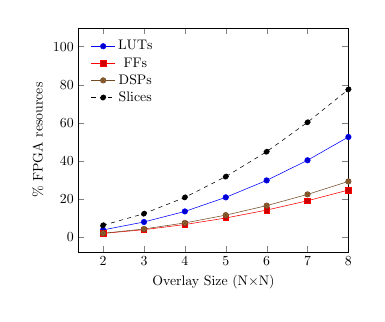
\begin{tikzpicture}[scale=0.5]
		\begin{axis}[
		xlabel=Overlay Size (N$\times$N),
		xtick = data,
		%xlabel near ticks,
		enlarge y limits = true,
		ylabel=$\%$ FPGA resources,
		ymax = 100,
		xmax = 8,
		legend pos=north west,
		legend style={draw=none}
		]
		\addplot plot coordinates {
			(2,     1910/532)
			(3,     4134/532)
			(4,     7087/532)
			(5,     11023/532)
			(6,     15761/532)
			(7,     21400/532)
			(8,     27918/532)
			
		};
		\addplot plot coordinates {
			(2,     1852/1064)
			(3,     3950/1064)
			(4,     6828/1064)
			(5,     10486/1064)
			(6,     14924/1064)
			(7,     20142/1064)
			(8,     26140/1064)
			
		};
		\addplot plot coordinates {
			(2,     4/2.2)
			(3,     9/2.2)
			(4,     16/2.2)
			(5,     25/2.2)
			(6,     36/2.2)
			(7,     49/2.2)
			(8,     64/2.2)
			
		};
		\addplot [mark=*, dashed] plot coordinates {
			(2,     802/133)
			(3,     1614/133)
			(4,     2754/133)
			(5,     4207/133)
			(6,     5948/133)
			(7,     8007/133)
			(8,     10306/133)
			
		};
		
		
		\legend{LUTs\\FFs\\DSPs\\Slices\\}
		\end{axis}
		\end{tikzpicture}
					
					
					
					%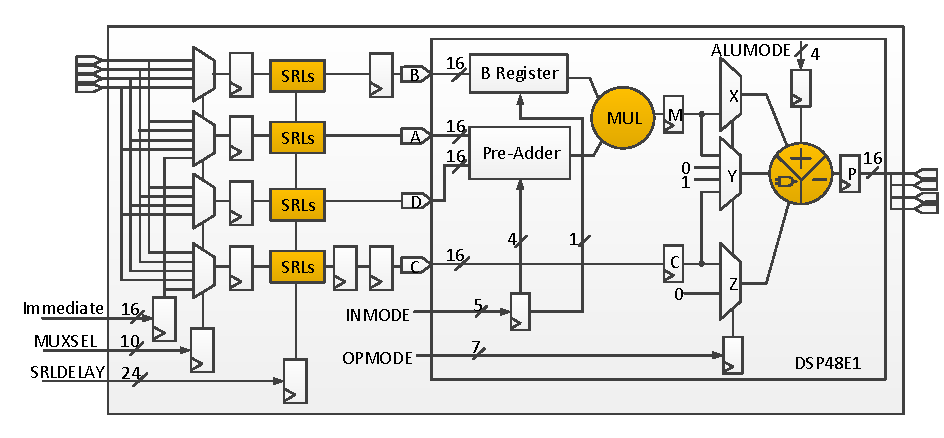
\includegraphics[width=26em]{fu_new}
				\end{center}    
				
			\end{minipage}
						\begin{minipage}{13em}
							\begin{center}      	
								
								
	 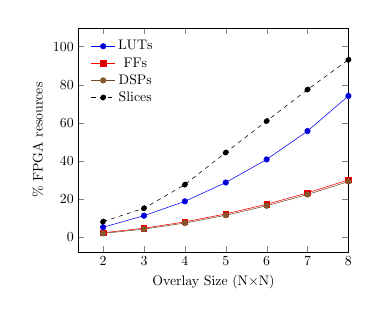
\begin{tikzpicture}[scale=0.5]
	 \begin{axis}[
	 xlabel=Overlay Size (N$\times$N),
	 ylabel=$\%$ FPGA resources,
	 enlarge y limits = true,
	 ymax = 100,
	 xmax = 8,
	 legend pos=north west,
	 legend style={draw=none}
	 ]
	 \addplot plot coordinates {
	 	(2,     2702/532)
	 	(3,     5927/532)
	 	(4,     9941/532)
	 	(5,     15198/532)
	 	(6,     21658/532)
	 	(7,     29599/532)
	 	(8,     39410/532)
	 	
	 };
	 \addplot plot coordinates {
	 	(2,     2296/1064)
	 	(3,     4866/1064)
	 	(4,     8382/1064)
	 	(5,     12844/1064)
	 	(6,     18252/1064)
	 	(7,     24606/1064)
	 	(8,     31906/1064)
	 	
	 };
	 \addplot plot coordinates {
	 	(2,     4/2.2)
	 	(3,     9/2.2)
	 	(4,     16/2.2)
	 	(5,     25/2.2)
	 	(6,     36/2.2)
	 	(7,     49/2.2)
	 	(8,     64/2.2)
	 	
	 };
	 \addplot [mark=*, dashed] plot coordinates {
	 	(2,     1067/133)
	 	(3,     2003/133)
	 	(4,     3655/133)
	 	(5,     5898/133)
	 	(6,     8097/133)
	 	(7,     10300/133)
	 	(8,     12379/133)
	 	
	 };
	 
	 
	 \legend{LUTs\\FFs\\DSPs\\Slices\\}
	 \end{axis}
	 \end{tikzpicture}
								
								%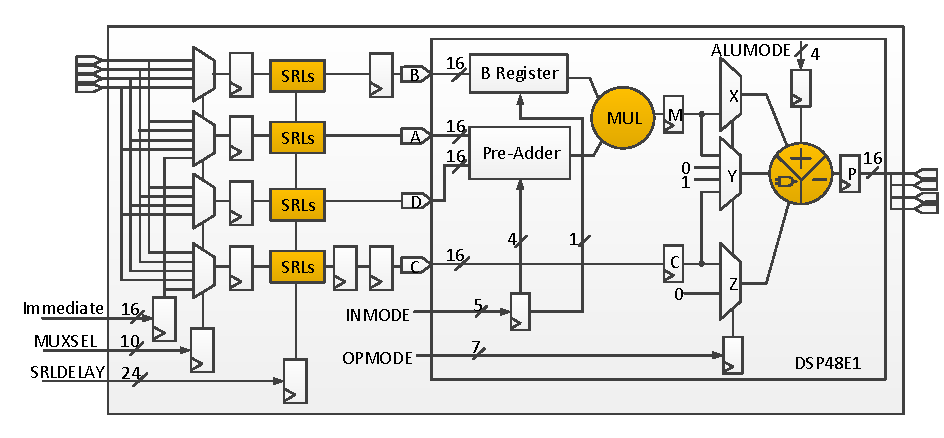
\includegraphics[width=26em]{fu_new}
							\end{center}    
							
						\end{minipage}

						\begin{minipage}{13em}
							\begin{center}      	
								
								
	 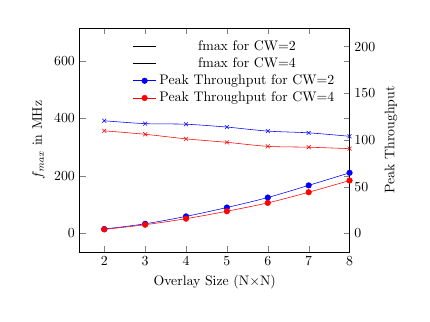
\begin{tikzpicture}[scale=0.5]
	 \begin{axis}[
	 xlabel=Overlay Size (N$\times$N),
	 ymin=0,
	 ymax=650,
	 enlarge y limits = true,
	 xmax = 8,
	 ylabel=$f_{\mathit{max}}$ in MHz,
	 legend pos=north east,
	 legend style={draw=none}
	 ]
	 \addplot[smooth,mark=x,blue]  plot coordinates {
	 	(2,     392)
	 	(3,     382)
	 	(4,     380)
	 	(5,     370)
	 	(6,     356)
	 	(7,     350)
	 	(8,     338)
	 	
	 };
	 \label{fmaxcw2}
	 
	 \addplot[smooth,mark=x,red]  plot coordinates {
	 	(2,     357)
	 	(3,     345)
	 	(4,     329)
	 	(5,     317)
	 	(6,     303)
	 	(7,     300)
	 	(8,     295)
	 	
	 };
	 \label{fmaxcw4}
	 %\legend{for CW=2\\for CW=4\\}
	 \end{axis}
	 \begin{axis}[%
	 ymin=0,ymax=200,
	 axis x line=none,
	 axis y line*=right,
	 xmax = 8,
	 enlarge y limits = true,
	 %	   xlabel near ticks,
	 %	   ylabel near ticks,
	 ylabel={Peak Throughput},
	 legend pos=north east,
	 legend style={draw=none}
	 ]
	 \addlegendimage{/pgfplots/refstyle=fmaxcw2}\addlegendentry{fmax for CW=2}
	 \addlegendimage{/pgfplots/refstyle=fmaxcw4}\addlegendentry{fmax for CW=4}
	 \addplot[smooth,mark=*,blue] plot coordinates {
	 	(2,     4.70)
	 	(3,     10.31)
	 	(4,     18.24)
	 	(5,     27.75)
	 	(6,     38.44)
	 	(7,     51.45)
	 	(8,     64.89)
	 	
	 };
	 
	 \addplot[smooth,mark=*,red] plot coordinates {
	 	(2,     4.28)
	 	(3,     9.31)
	 	(4,     15.79)
	 	(5,     23.77)
	 	(6,     32.72)
	 	(7,     44.10)
	 	(8,     56.64)
	 	
	 };
	 \addlegendentry{Peak Throughput for CW=2}\addlegendentry{Peak Throughput for CW=4}
	 %\legend{Peak Throughput for CW=2\\Peak Throughput for CW=4\\}
	 \end{axis}
	 \end{tikzpicture}
							\end{center}    
							
						\end{minipage}
						
			
		}
	}
\end{center}


